\documentclass[11pt]{article}
\usepackage[utf8]{inputenc}
\usepackage{siunitx}
\usepackage{preamble}
\usepackage{graphicx}
\usepackage{pdfpages}
\newcommand{\polar}[0]{PolaRx5\textsuperscript{TR}}
\newcommand{\BNC}[0]{Berkeley Nucleonics 1105}
%\usepackage[margin=1in]{geometry}



\begin{document}
\maketitle

\addtocounter{page}{-1}
\pagenumbering{roman}
\thispagestyle{empty}
%~~~~~~~~~~~~~~~~~~~~~~~~~~~~~~~~~~~~~~~~~~~~~~~~~~~~~~~~~~~~~~~~~~~~~~~~~~~~~~~~~~~~~~~~~~~~~~~
%\newpage

%\null\vspace{2in}
%\begin{abstract}
%\blindtext 
%\end{abstract}
%\vspace{\fill}
%\thispagestyle{empty}

\newpage
\tableofcontents


\newpage
\section*{Revision History}

\begin{table}[h]
    \centering
    \begin{tabular}{|c|c|c|c|}
        \hline
        Version & Date & Who & Changes's description\\
        \hline
        0 & April 2024 & DAL  & First version, all new\\
        \hline
    \end{tabular}
\end{table}

\newpage
\section*{List of Acronyms}

\begin{table}[ht]
\centering
\begin{tabular}[t]{ll}
\hline
CAB DLY & Delay in the antenna cable\\
DUT & Device Under Test\\
CGGTTS &  Common GNSS Generic Time Transfer Standard \\
GNSS & Global Navigation Satellite System\\
GPS & Global Positioning System\\
INT DLY & Internal delay of GNSS receiver\\ 
INTI & Instituto Nacional de Tecnolog\'ia Industrial\\
PPS & Pulse per second \\
REF DLY & Delay of the cable between the reference point and the PPS-in connector of a receiver\\
RINEX & Receiver Independent Exchange \\
SIM & Sistema Interamericano de Metrolog\'ia\\
TDEV & Time deviation\\
UTC & Coordinated Universal Time\\
\hline
\end{tabular}
\caption{Acronyms used in this procedure}
\end{table}%

%\newpage
%\section*{Conventions and Notation}\label{Conventions}
%\addcontentsline{toc}{subsection}{\textit{Conventions and Notation}}
%\vspace{2em}

%\listoffigures
%\addcontentsline{toc}{subsection}{\textit{List of Figures}}
%\vspace{2em}

%\listoftables
%\addcontentsline{toc}{subsection}{\textit{List of Tables}}
%\vspace{2em}
%\newpage

%\section*{Acknowledgements}\label{Acknowledgements}
%\addcontentsline{toc}{subsection}{\textit{Acknowledgements}}
%\vspace{2em}

%\section*{Preface}\label{Preface}
%\addcontentsline{toc}{subsection}{\textit{Preface}}
%\vspace{2em}

%~~~~~~~~~~~~~~~~~~~~~~~~~~~~~~~~~~~~~~~~~~~~~~~~~~~~~~~~~~~~~~~~~~~~~~~~~~~~~~~~~~~~~~~~~~~~~~~
%Main Content sections start

\newpage
\pagenumbering{arabic}
\part{Traveling System Operator Manual}
%\addcontentsline{toc}{part}{Main Content}

%~~~~~~~~~~~~~~~~~~~~~~~~~~~~~~~~~~~~~~~~~~~~~~~~~~~~~~~~~~~~~~~~~~~~~~~~~~~~~~~~~~~~~~~~~~~~~~~

\section{Overview}

The current procedure follows as much as possible the documents  \textit{BIPM guidelines for GNSS calibration} \cite{guidelines} and \textit{How to get GNSS calibration for UTC(k) laboratories} \cite{getcal}.

As mentioned in \cite{guidelines}, \textit{All laboratories contributing to UTC are equipped with GNSS receivers, almost all of them providing the official time link, either by one-technique links (GPS or Galileo) [...]. The characterization of the delays in the time transfer equipment (here referred to as “calibration”) is essential to
the accuracy of time transfer and time dissemination. The set of GNSS equipment in laboratories used for time
transfer in UTC needs to be calibrated, and the system is to be maintained through a programme of repeated calibrations over time.}

The calibration of a time and frequency station includes the measurement of several delays. They are depicted in figure \ref{fig:delays} and explained afterwards.

\begin{figure}[ht]
\begin{center}
\fbox{	
\tikzset{arrow/.style={-stealth, thick, draw=gray!80!black}}

\begin{tikzpicture}[ampersand replacement=\&]

\node[text width=3cm] at (0.7,0.75) 
    {Antenna};
\node[text width=3cm] at (5.5,0.75) 
    {Receiver};
\node[text width=2.5cm] at (10,1) 
    {Time Reference};


%    \node[rectangle, rounded corners, draw, fill=gray!20, minimum height=1cm] at (0,0) (A) {\textsc{Novatel 750}};	
%    \node[rectangle, rounded corners, draw, fill=gray!20, minimum height=1cm] at (5,0) (R) {\textsc{Polar5xTR}};      
%    \node[rectangle, rounded corners, draw, fill=gray!20, minimum height=1cm] at (10,0) (C) {\textsc{UTC(local)}};


\node[rectangle, rounded corners, draw, fill=gray!20, minimum height=1cm, minimum width=2.5cm] at (0,0) (A) {\textsc{      }};	
\node[rectangle, rounded corners, draw, fill=gray!20, minimum height=1cm, minimum width=2.3cm] at (5,0) (R) {\textsc{      }};      
\node[rectangle, rounded corners, draw, fill=gray!20, minimum height=1cm, minimum width=2cm] at (10,0) (C) {\textsc{UTC(local)}};



\draw [-] (5,-0.5) -- (5,-0.6) node [midway, below] {\scriptsize PPS out};
\draw [|-|, draw=blue] (0,-1.5) -- (1.3,-1.5) node [midway, fill=white,text=blue] {$X_{S,i}$};
\draw [|-|] (1.3,-1) -- (3.8,-1) node [midway, fill=white] {$X_{C}+ X_{D}$};
\draw [|-|, draw=blue] (3.8,-1.5) -- (5,-1.5) node [midway, fill=white, text=blue] {$X_{R,i}$};
\draw [|-|] (5,-2) -- (6.2,-2) node [midway, fill=white] {$X_{0}$};
\draw [|-|] (6.2,-1) -- (8.8,-1) node [midway, fill=white] {$X_{P}$};



\draw [|-|] (5,-3) -- (8.8,-3) node [midway, above] {\textsc{REFDLY} $= X_{0} + X_{P}$};
\draw [|-|] (1.3,-3) -- (3.8,-3) node [midway, above] {CABDLY $= X_{C} + X_{D}$};

\node[text width=4cm, text=blue] at (4.5,-4) (O) {\textsc{INTDLY} = $X_{S,i} + X_{R,i}$};
 
\path[arrow] (A) edge (R)
(C) edge (R)
;

%\path[arrow, dotted, draw = blue] (C) edge (R)
%;


\end{tikzpicture}
}
\caption{Definition of delays in a receiver station}
\label{fig:delays}
\end{center}
\end{figure}



\begin{enumerate}
    \item \textbf{INT DLY} The sum $X_R + X_S$ represents the “INT DLY” field in the CGGTTS header:
$X_R$ represents the receiver hardware delay, between a reference point whose definition depends on the receiver type and the internal time reference of the measurements. $X_S$ represents the antenna delay, between the phase center and the antenna cable connector at the antenna body. We distinguish the two quantities for the two GPS frequencies, f1 and f2. %INT DLY(f1) and INT DLY(f2) of receiver V are the basic quantities that are determined during the relative calibration. For calculating ionosphere—free observation data, INT DLY(f3) is calculated as 2.54 $\times $INT DLY(f1) - 1.54$\times $INT DLY(f2) for GPS, and as 2.26$\times $INT DLY(f1) - 1.26$\times $INT DLY(f2) for Galileo, respectively. In figures and results tables we use the designation P1, P2 for GPS.%, and E1, E5a for Galileo, instead of f1, f2.

The following terms are considered frequency independent, i. e. no distinction is made for f1 and f2.

\item \textbf{CAB DLY}
The sum $X_C + X_D$ represents the “CAB DLY” field in the CGGTTS header.
$X_C$ corresponds to the delay of the long cable from the antenna to the input connector at either the antenna splitter or the receiver body directly. If a splitter is installed, $X_D$ corresponds to the delay of the splitter and the small cable up to the receiver body. For a simple set-up with just an 
antenna cable, $X_D = 0$.

\item \textbf{REF DLY}
The sum $X_P + X_O$ represents the “REF DLY” field in the CGGTTS header. $X_P$ corresponds to the delay of the cable between the laboratory reference point for local UTC and the 1 PPS-in connector of the receiver. 

\end{enumerate}

CABDLY and $X_P$ are delays generated by cables which have to be measured by the visited laboratory.\\
The internal delay of the visited receiver will be determined by with the use of the  traveling receiver and using the zero-baseline technique. (Figure \ref{fig:zerobaseline})


\begin{figure}[ht]
\begin{center}
\tikzset{arrow/.style={-stealth, thick, draw=gray!80!black}}

\begin{tikzpicture}[ampersand replacement=\&]

\node[text width=3cm] at (0.3,0.75) 
    {Antenna};
\node[text width=3cm] at (5.2,0.75) 
    {Receiver};
\node[text width=2.5cm] at (10,0) 
    {Time Reference};

\node[rectangle, rounded corners, draw, fill=gray!20, minimum height=1cm, minimum width=2.5cm] at (0,0) (A) {\textsc{Novatel 750}};	
\node[rectangle, rounded corners, draw, fill=gray!20, minimum height=1cm, minimum width=2.3cm] at (5,0) (R) {\textsc{PolaRx5TR}};      
\node[rectangle, rounded corners, draw, fill=gray!20, minimum height=1cm, minimum width=2cm] at (10,-1) (C) {\textsc{UTC(local)}};


\node[text width=3cm] at (0.3,-1.25) 
    {Local Antenna};
\node[text width=3cm] at (5.2,-1.25) 
    {Local Receiver};


\node[rectangle, rounded corners, draw, fill=gray!20, minimum height=1cm, minimum width=2.5cm] at (0,-2) (B) {\textsc{      }};	
\node[rectangle, rounded corners, draw, fill=gray!20, minimum height=1cm, minimum width=2.5cm] at (5,-2) (S) {\textsc{      }};      

 
\path[arrow] (A) edge (R)
(C) edge (R)
(B) edge (S)
(C) edge (S)
;

\end{tikzpicture}

\caption{Zero baseline measurement}
\label{fig:zerobaseline}
\end{center}
\end{figure}

The difference of the total delay for a pair of co-located receivers is the sum of the delays incurred in the antenna cable (CABDLY) and the internal delay(INTDLY), minus the time offset at the latching
point of the receiver as referenced to a fixed point, usually UTC(k)(REFDLY). The internal delay
is comprised of both code- and frequency-dependent delays in the antenna and the receiver. After
accounting for the baseline geometry, the difference in pseudoranges between a pair of receivers, say
for P1, is given by

\begin{equation}
 RAWDIF(P1)_{A-B} = \Delta CABDLY_{A-B} + \Delta INTDLY_{A-B} - \Delta REFDLY_{A-B}
\end{equation}

\section{Equipment}
The SIM traveling is composed of the elements depicted in table \ref{tab:elements}.



\begin{table}[h]
    \centering
    \begin{tabular}{cllc}
       Quantity & Element & Model & Serial Number\\
       \hline
        1       & Laptop              & Dell Latitude 7300        & 9SVR2R2 \\
        1       & GNSS Receiver       & PolaRx5TR                 & 4701626\\
        1       & Frequency Counter   & Berkeley Nucleonics 1105  & TW00048101\\
        1       & GNSS Antenna        & Novatel GNSS 750          & 10200001 \\
        1       & Antenna Cable       & LMR LW400                 & - \\
        2       & Cable               & LMR 240                   & -\\
        1       & Case& Pelican 1690 Case & -\\
    \end{tabular}
    \caption{System's elements.}
    \label{tab:elements}
\end{table}

\subsection{SIM laptop}
Please use the following to log in to the SIMr travelling System laptop:

Username: denali

Password: nistg2cal

\subsection{Antenna}

\begin{minipage}{0.75\textwidth}
A robust pillar or mount with a 5/8" x 11 thread that extends between 3/8" and 7/8" (9 mm and 22 mm)  is required to set up the antenna. The weight of the antenna is \SI{7.6}{\kilo\gram}. Please consider this fact when mounting it. Make sure the antenna has a clear view of the sky.


Connect one end of the antenna cable to the antenna
and the other end to the rear-panel ‘Main’ socket on
the PolaRx5TR. 
\end{minipage}
\begin{minipage}{0.25\textwidth}
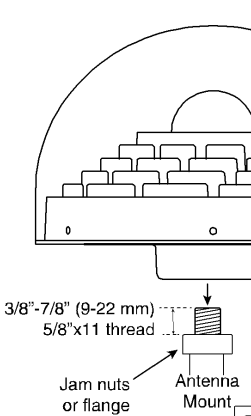
\includegraphics[width=0.9\linewidth]{Figures/antenamount}
Antenna mount. (From GNSS 750 manual)
\end{minipage}

\subsection{Frequency Counter}
The traveling frequency counter must be referenced the local \SI{10}{\mega\hertz} reference.



\subsection{GNSS receiver}


%~~~~~~~~~~~~~~~~~~~~~~~~~~~~~~~~~~~~~~~~~~~~~~~~~~~~~~~~~~~~~~~~~~~~~~~~~~~~~~~~~~~~~~~~~~~~~~~




\part{Measurement Procedure }

\section{Cable Delays Measurements}

The visited laboratory must inform CABDLY and REFDLY of the local receiver. This means that the laboratory will have to determine the delay of two cables and (depending on the receiver model), the value of $X_0$.
The method sugested for this measurements is the depicted in figure \ref{fig:DUTdelaymeasurement}.


\begin{figure}[ht]
\begin{center}

\tikzset{arrow/.style={-stealth, thick, draw=gray!80!black}}

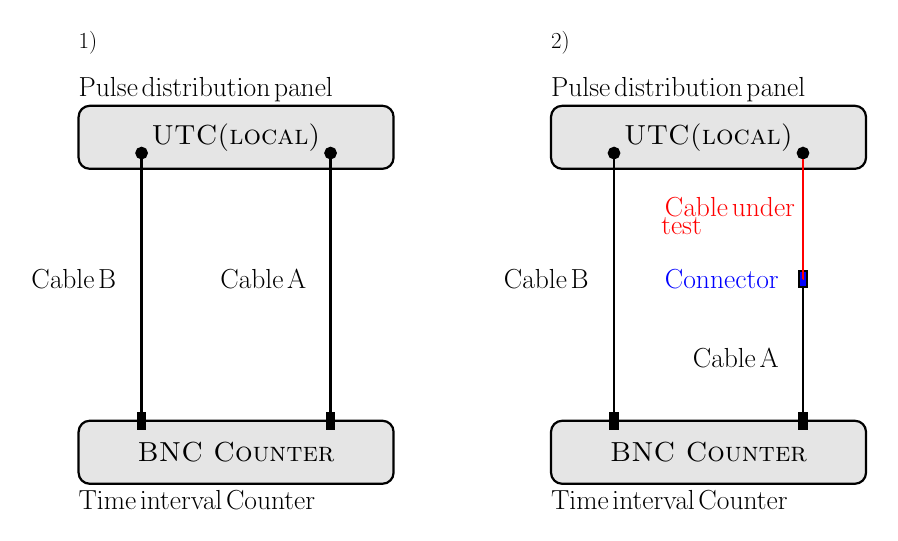
\begin{tikzpicture}[thick,scale=0.4, every node/.style={scale=0.4}]

%% PRIMERA MEDICION
\node[text width=10cm] at (0,3) 
{\huge{1)}};
\node[text width=10cm] at (0,1.5) 
{\Huge{Pulse distribution panel}};

% Distribuidor de pulsos
\node[rectangle, rounded corners, draw, fill=gray!20, minimum height=2cm, minimum width=10cm] at (0,0) (Dist) {\textsc{\Huge{UTC(local)}}};

% Contador
\node[text width=10cm] at (0,-11.5) 
{\Huge{Time interval Counter}};
\node[rectangle, rounded corners, draw, fill=gray!20, minimum height=2cm, minimum width=10cm] at (0,-10) (Count) {\textsc{\Huge{BNC Counter}}};

% Canales distribuidor
\node[circle, draw, fill=black, minimum height=.3cm, minimum width=0.2cm] at (-3,-0.5) (PPS1) {   };

\node[circle, draw, fill=black, minimum height=.3cm, minimum width=0.2cm] at (3,-0.5) (PPS2) {   };

% Canales contador
\node[rectangle, draw, fill=black, minimum height=.5cm, minimum width=0.2cm] at (-3,-9) (Ch1) {   };
\node[rectangle, draw, fill=black, minimum height=.5cm, minimum width=0.2cm] at (3,-9) (Ch2) {   };

% Cables
\draw[-] (PPS1) |- (Ch1);
\draw[-] (PPS2) |- (Ch2);

\node[text width=5cm] at (-4,-4.5) 
{\Huge{Cable B}};

\node[text width=5cm] at (2,-4.5) 
{\Huge{Cable A}};


%% SEGUNDA MEDICION
\node[text width=10cm] at (15,3) 
{\huge{2)}};
\node[text width=10cm] at (15,1.5) 
{\Huge{Pulse distribution panel}};

% Distribuidor de pulsos
\node[rectangle, rounded corners, draw, fill=gray!20, minimum height=2cm, minimum width=10cm] at (15,0) (Dist) {\textsc{\Huge{UTC(local)}}};

% Contador
\node[text width=10cm] at (15,-11.5) 
{\Huge{Time interval Counter}};
\node[rectangle, rounded corners, draw, fill=gray!20, minimum height=2cm, minimum width=10cm] at (15,-10) (Count) {\textsc{\Huge{BNC Counter}}};

% Canales distribuidor
\node[circle, draw, fill=black, minimum height=.3cm, minimum width=0.2cm] at (12,-0.5) (2PPS1) {   };

\node[circle, draw, fill=black, minimum height=.3cm, minimum width=0.2cm] at (18,-0.5) (2PPS2) {   };

% Canales contador
\node[rectangle, draw, fill=black, minimum height=.5cm, minimum width=0.2cm] at (12,-9) (2Ch1) {   };
\node[rectangle, draw, fill=black, minimum height=.5cm, minimum width=0.2cm] at (18,-9) (2Ch2) {   };

%Conector
\node[rectangle, draw, fill=blue, minimum height=.5cm, minimum width=0.2cm] at (18,-4.5) (2Tube) {   };
\node[text width=5cm] at (16,-4.5) 
{\Huge{ \textcolor{blue}{ Connector}}};

% Cables
\draw[-] (2PPS1) |- (2Ch1);
\draw[-, draw = red] (2PPS2) |- (2Tube);
\draw[-] (2Tube) |- (2Ch2);


\node[text width=5cm] at (11,-4.5) 
{\Huge{Cable B}};
\node[text width=5cm] at (17,-7) 
{\Huge{Cable A}};
\node[text width=5cm] at (16,-2.5) 
{\Huge{ \textcolor{red}{ Cable under test}}};





\end{tikzpicture}
\caption{Measurement sequence for the determination of delays.} \label{fig:DUTdelaymeasurement}
\end{center}
\end{figure}

Measurement 1) corresponds to a tare. Then the cable under test and a connector must be added to the channel 2 of the time interval counter. The measurement equation for this procedure is 

\begin{equation}
Delay = Delay2 - Delay1 + corrections
\end{equation}
The corrections are the estimated delay introduced by adaptator: \SI{-0.1}{\nano\second}. 


Cable delays must be measured using the counter included in the traveling system. By enabling the "RECALL 1" memory, 100 time interval measurements are done. To do this, press the \textit{SAVE \& RECALL} button from the front panel of the counter. Then select \textit{Recall} and option 1 (This should be the only memory stored). Then press \textit{Run Recall}.

In this configuration, a \SI{1}{\volt} trigger level is applied on both channels, together with a DC coupling and a \SI{50}{\ohm} impedance.


The display will present the mean value of the delay between Channel 1 and Channel2, averaged over 100 measurements. The standard deviation is also shown.

If you cannot unmount the antenna cable to perform this measurement, please contact \texttt{\url{luna@inti.gob.ar}}.

%\subsection{$X_p$ Measurement}
%\subsection{CABDLY Measurement}
%The method to measure the delay introduced by the antenna cable is the same as the one used to measure the delay 

\section{GNSS measurements with SIMr receiver}
\subsection{REF DLY ($X_0$ + $X_P$) Measurement}
Before starting logging data of the traveling receiver, it is necessary to measure the value of the phase relationship between the \SI{10}{\mega\hertz} reference and the 1PPS input (REF DLY). For that:

\begin{enumerate}
    \item Connect the antenna cable, \SI{10}{\mega\hertz} reference and the 1 PPS to the \polar receiver as shown in figure \ref{fig:cggttsdelays.png}
    
    \begin{figure}[ht]
    \begin{center}
    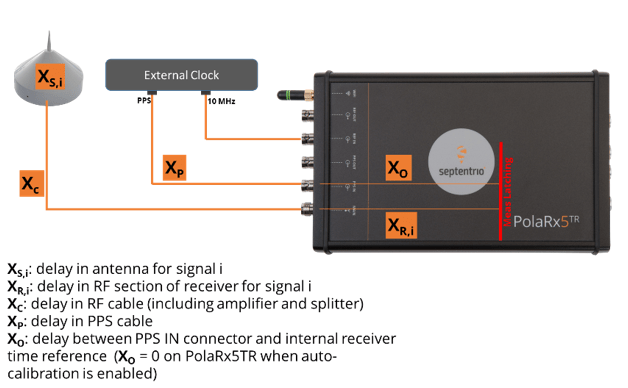
\includegraphics[width=0.8\linewidth]{./Figures/cggttsdelays.png}
    \caption{\polar connections. From receiver user-interface. } \label{fig:cggttsdelays.png}
    \end{center}
    \end{figure}

    
    \item Power the receiver on.
    \item Connect Cable A to PPS out of \polar. Switch the receiver power. Wait for a few minutes for the receiver to lock with the external reference. A stable output of the TIC is indicative of a firm lock.
    \item Turn on the WiFi by firmly ressing the front-panel WiFi button to turn on the WiFi modem.
    \item Find the \polar WiFi signal on the SIM laptop and click: \textbf{Connect}
    \item When connected, open the web browser and go to the ip 192.168.20.1
    \item Check if the \polar is tracking satellites by selecting the 'GNSS' tab and then 'Satellites and Signals'. The SIMr should track between 15 and 25 GPS and Glonass satelites. The Carrier-to-Noise plot for the GPS should show about 3 satellites with an L1CA above 50 dB-Hz.
\end{enumerate}

\begin{figure}[ht]
\begin{center}

%\tikzset{arrow/.style={-stealth, thick, draw=gray!80!black}}

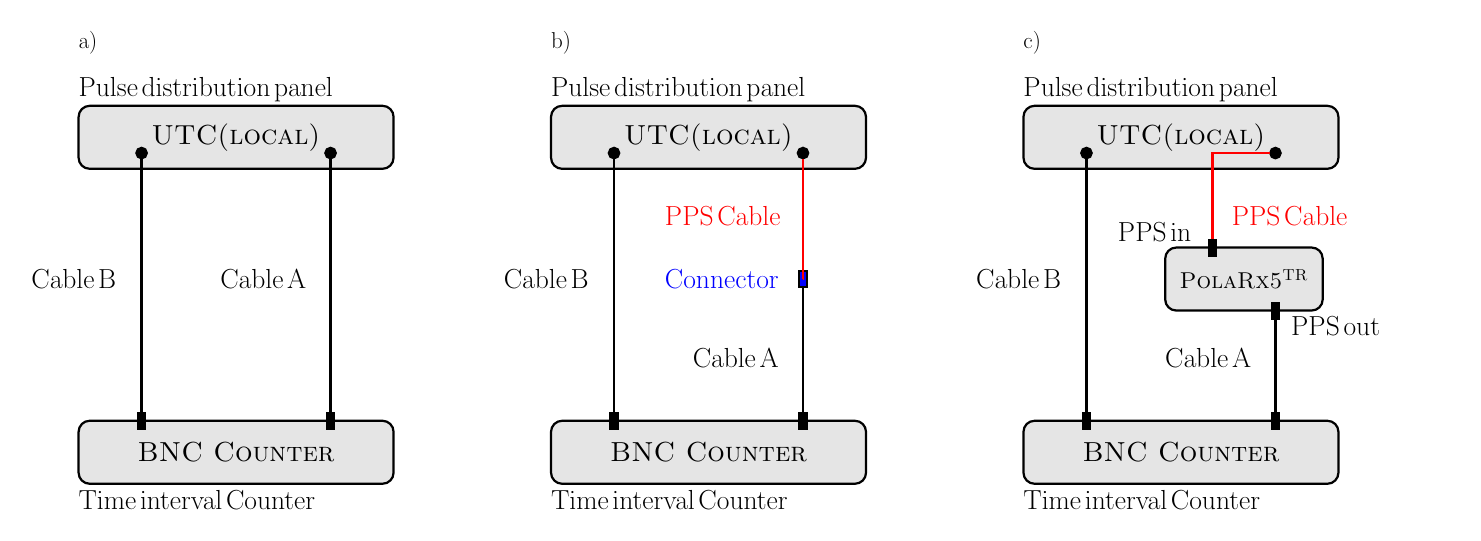
\begin{tikzpicture}[thick,scale=0.4, every node/.style={scale=0.4}]

%% PRIMERA MEDICION
\node[text width=10cm] at (0,3) 
{\huge{a)}};
\node[text width=10cm] at (0,1.5) 
{\Huge{Pulse distribution panel}};

% Distribuidor de pulsos
\node[rectangle, rounded corners, draw, fill=gray!20, minimum height=2cm, minimum width=10cm] at (0,0) (Dist) {\textsc{\Huge{UTC(local)}}};

% Contador
\node[text width=10cm] at (0,-11.5) 
{\Huge{Time interval Counter}};
\node[rectangle, rounded corners, draw, fill=gray!20, minimum height=2cm, minimum width=10cm] at (0,-10) (Count) {\textsc{\Huge{BNC Counter}}};

% Canales distribuidor
\node[circle, draw, fill=black, minimum height=.3cm, minimum width=0.2cm] at (-3,-0.5) (PPS1) {   };

\node[circle, draw, fill=black, minimum height=.3cm, minimum width=0.2cm] at (3,-0.5) (PPS2) {   };

% Canales contador
\node[rectangle, draw, fill=black, minimum height=.5cm, minimum width=0.2cm] at (-3,-9) (Ch1) {   };
\node[rectangle, draw, fill=black, minimum height=.5cm, minimum width=0.2cm] at (3,-9) (Ch2) {   };

% Cables
\draw[-] (PPS1) |- (Ch1);
\draw[-] (PPS2) |- (Ch2);

\node[text width=5cm] at (-4,-4.5) 
{\Huge{Cable B}};

\node[text width=5cm] at (2,-4.5) 
{\Huge{Cable A}};


%% SEGUNDA MEDICION
\node[text width=10cm] at (15,3) 
{\huge{b)}};
\node[text width=10cm] at (15,1.5) 
{\Huge{Pulse distribution panel}};

% Distribuidor de pulsos
\node[rectangle, rounded corners, draw, fill=gray!20, minimum height=2cm, minimum width=10cm] at (15,0) (Dist) {\textsc{\Huge{UTC(local)}}};

% Contador
\node[text width=10cm] at (15,-11.5) 
{\Huge{Time interval Counter}};
\node[rectangle, rounded corners, draw, fill=gray!20, minimum height=2cm, minimum width=10cm] at (15,-10) (Count) {\textsc{\Huge{BNC Counter}}};

% Canales distribuidor
\node[circle, draw, fill=black, minimum height=.3cm, minimum width=0.2cm] at (12,-0.5) (2PPS1) {   };

\node[circle, draw, fill=black, minimum height=.3cm, minimum width=0.2cm] at (18,-0.5) (2PPS2) {   };

% Canales contador
\node[rectangle, draw, fill=black, minimum height=.5cm, minimum width=0.2cm] at (12,-9) (2Ch1) {   };
\node[rectangle, draw, fill=black, minimum height=.5cm, minimum width=0.2cm] at (18,-9) (2Ch2) {   };

%Conector
\node[rectangle, draw, fill=blue, minimum height=.5cm, minimum width=0.2cm] at (18,-4.5) (2Tube) {   };
\node[text width=5cm] at (16,-4.5) 
{\Huge{ \textcolor{blue}{ Connector}}};

% Cables
\draw[-] (2PPS1) |- (2Ch1);
\draw[-, draw = red] (2PPS2) |- (2Tube);
\draw[-] (2Tube) |- (2Ch2);


\node[text width=5cm] at (11,-4.5) 
{\Huge{Cable B}};
\node[text width=5cm] at (17,-7) 
{\Huge{Cable A}};
\node[text width=5cm] at (16,-2.5) 
{\Huge{ \textcolor{red}{ PPS Cable}}};


%% TERCERA MEDICION

\node[text width=10cm] at (30,3) 
{\huge{c)}};
\node[text width=10cm] at (30,1.5) 
{\Huge{Pulse distribution panel}};

% Distribuidor de pulsos
\node[rectangle, rounded corners, draw, fill=gray!20, minimum height=2cm, minimum width=10cm] at (30,0) (Dist) {\textsc{\Huge{UTC(local)}}};

% Contador
\node[text width=10cm] at (30,-11.5) 
{\Huge{Time interval Counter}};
\node[rectangle, rounded corners, draw, fill=gray!20, minimum height=2cm, minimum width=10cm] at (30,-10) (Count) {\textsc{\Huge{BNC Counter}}};

% Receptor

\node[rectangle, rounded corners, draw, fill=gray!20, minimum height=2cm, minimum width=5cm] at (32,-4.5) (polar) {\textsc{\huge{\polar}}};

% PPS in & out
\node[rectangle, draw, fill=black, minimum height=.5cm, minimum width=0.2cm] at (31,-3.5) (PPSin) { };
\node[rectangle, draw, fill=black, minimum height=.5cm, minimum width=0.2cm] at (33,-5.5) (PPSout) { };
\node[text width=5cm] at (30.5,-3) 
{\Huge{PPS in}};
\node[text width=5cm] at (36,-6) 
{\Huge{PPS out}};

% Canales distribuidor
\node[circle, draw, fill=black, minimum height=.3cm, minimum width=0.2cm] at (27,-0.5) (3PPS1) {   };

\node[circle, draw, fill=black, minimum height=.3cm, minimum width=0.2cm] at (33,-0.5) (3PPS2) {   };

% Canales contador
\node[rectangle, draw, fill=black, minimum height=.5cm, minimum width=0.2cm] at (27,-9) (3Ch1) {   };
\node[rectangle, draw, fill=black, minimum height=.5cm, minimum width=0.2cm] at (33,-9) (3Ch2) {   };

% Cables
\draw[-] (3PPS1) |- (3Ch1);
\draw[-, draw = red] (3PPS2) -| (PPSin);
\draw[-] (PPSout) |- (3Ch2);


\node[text width=5cm] at (26,-4.5) 
{\Huge{Cable B}};
\node[text width=5cm] at (32,-7) 
{\Huge{Cable A}};
\node[text width=5cm] at (34,-2.5) 
{\Huge{ \textcolor{red}{ PPS Cable}}};




\end{tikzpicture}
\caption{Measurement sequence for the determination of the value of phase relationship between the \SI{10}{\mega\hertz} reference and the 1PPS input ($X_0$). The "PPS cable " is not part of the traveling system.} \label{fig:cabledelaymeasurement}
\end{center}
\end{figure}

Please fill the table \textit{Annex: REF DLY measurement} of the Appendix with the measurement results of steps a), b) and c) in figure \ref{fig:cabledelaymeasurement}



\subsection{RAWDIFF Measurement}
%\addcontentsline{toc}{part}{Main Content}
Once in the webpage of the \polar, follow these steps to start a measurement:

\begin{itemize}
    \item In the \textit{Timing} section, make sure the option \textit{Enable compensation of PPSIN internal delay} is OFF.
    \item Go to the \textit{Logging} section and then click on the \textit{Log Sessions} option.
    \item Then click on the \textit{Create} button on any unused Log session.
    \item In the Edit Session section, assign a Session Name to the measurement.
    \item Go to the RINEX tab and click on the \textit{Configure RINEX Logging} button. In this menu, select the GNSS measurements to log (usually only GPS constellation is enough) and click OK. In the \textit{RINEX file duration} option, select 24 hours. For \textit{Observation interval}, select 30 seconds.
    \item Go to the CGGTTS tab and go to \textit{Configure CGGTTS logging}. Select the GNSS constellation to log CGGTTS for (usually only GPS constellation is enough) and click OK.
    \item Finally, press OK on the \textit{Edit Session LOG} menu.
\end{itemize}

After these steps, an active log session should be visible. (Figure \ref{fig:screenPolar4}).

After a few minutes, go to the \textit{Logging} and select \textit{Disk Contents}. You should see there the ongoing measurement. From the same menu, you will be able to download the data to the laptop after the 10 days of measurement.  



   \begin{figure}[ht]
    \begin{center}
    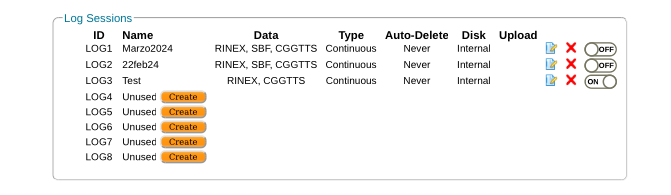
\includegraphics[width=1\linewidth]{./Figures/screenPolar4.png}
    \caption{\polar connections. From receiver user-interface. } \label{fig:screenPolar4}
    \end{center}
    \end{figure}



%~~~~~~~~~~~~~~~~~~~~~~~~~~~~~~~~~~~~~~~~~~~~~~~~~~~~~~~~~~~~~~~~~~~~~~~~~~~~~~~~~~~~~~~~~~~~~~~
\newpage
\appendix
\renewcommand{\thesection}{\Alph{section}}
\renewcommand{\thesubsection}{\roman{subsection}}
\renewcommand{\theequation}{A-\arabic{equation}}


%~~~~~~~~~~~~~~~~~~~~~~~~~~~~~~~~~~~~~~~~~~~~~~~~~~~~~~~~~~~~~~~~~~~~~~~~~~~~~~~~~~~~~~~~~~~~~~~



%~~~~~~~~~~~~~~~~~~~~~~~~~~~~~~~~~~~~~~~~~~~~~~~~~~~~~~~~~~~~~~~~~~~~~~~~~~~~~~~~~~~~~~~~~~~~~~~
\newpage
\part*{References}

\begin{thebibliography}{9}

\bibitem{Rovera}
Rovera, D., Abgrall, M., Uhrich, P., \& Siccardi, M. (2015, April). Techniques of antenna cable delay measurement for GPS time transfer. In 2015 Joint Conference of the IEEE International Frequency Control Symposium \& the European Frequency and Time Forum (pp. 239-244). IEEE.

\bibitem{dclrinex}
\url{ftp://ftp2.bipm.org/pub/tai/publication/gnss-calibration/doc-soft/}

\bibitem{guidelines}
\url{https://webtai.bipm.org/ftp/pub/tai/publication/gnss-calibration/guidelines/bipmcalibration_guidelines_v40.pdf}

\bibitem{getcal}
\url{https://webtai.bipm.org/ftp/pub/tai/publication/gnss-calibration/guidelines/How-to-get-calibration-March2024.pdf}

\bibitem{GUMintro}
BIPM, IEC, IFCC, ILAC, ISO, IUPAC, IUPAP, and OIML. Evaluation of measurement data — An introduction to the “Guide to the expression of uncertainty in measurement” and related documents.
Joint Committee for Guides in Metrology, JCGM 104:2009. \url{https://www.bipm.org/documents/20126/2071204/JCGM_104_2009.pdf/19e0a96c-6cf3-a056-4634-4465c576e513}

\bibitem{GUM}
JCGM 100:2008: Evaluation of measurement data — Guide to the expression of uncertainty in measurement \url{https://www.bipm.org/documents/20126/2071204/JCGM_100_2008_E.pdf/cb0ef43f-baa5-11cf-3f85-4dcd86f77bd6}

\bibitem{CircularT}
\url{https://webtai.bipm.org/ftp/pub/tai/Circular-T/cirt/cirt.434}

\bibitem{explanatory}
\url{https://webtai.bipm.org/ftp/pub/tai/other-products/notes/explanatory_supplement_v0.6.pdf}

\end{thebibliography}

\part*{Appendices}
%\addcontentsline{toc}{part}{Appendices}
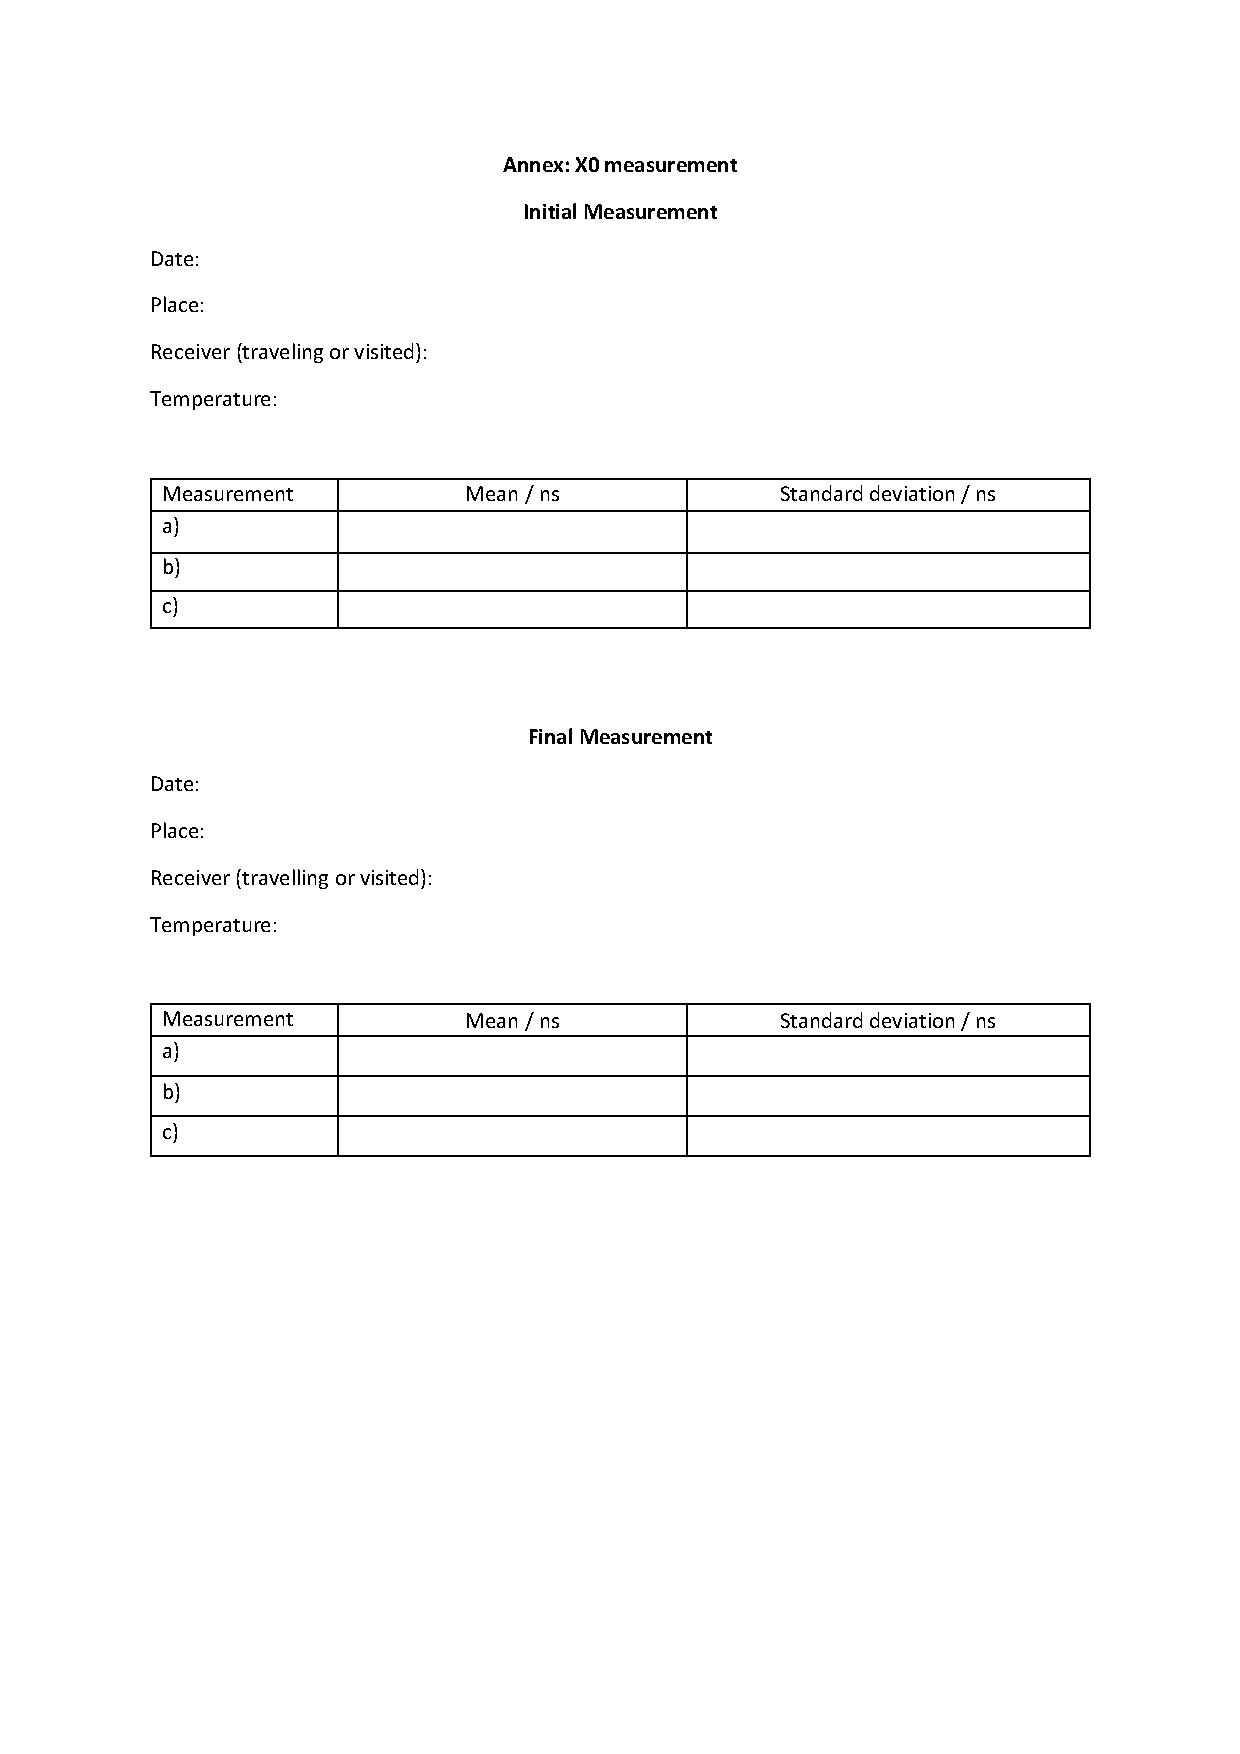
\includepdf[pages=-]{./PlanillaCalibracionX0SIM.pdf}

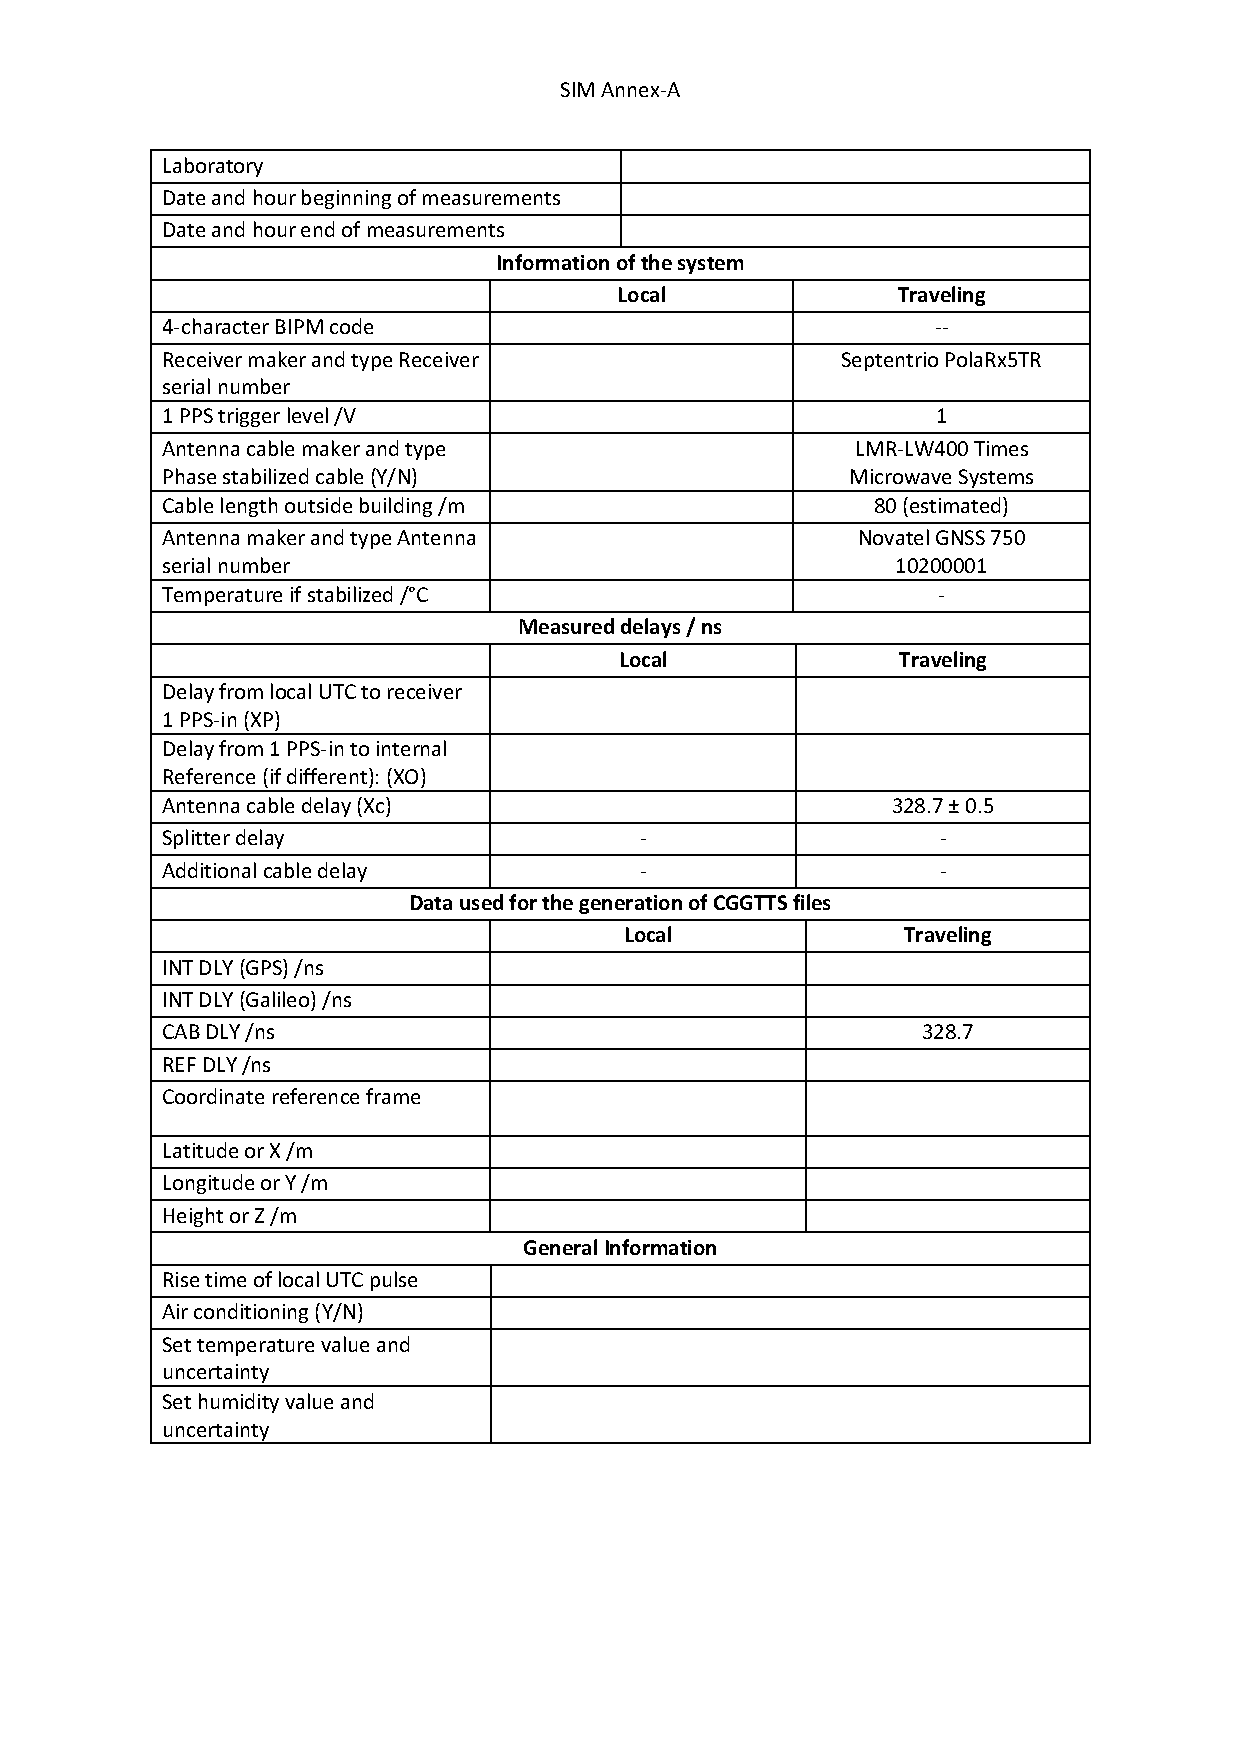
\includepdf[pages=-]{./PlanillaCalibracionReceptorSIM.pdf}




\end{document}

